\documentclass[11pt,a4paper]{article}
\usepackage[utf8]{inputenc}
\usepackage{amsmath,amssymb,amsthm}
\usepackage{algorithm}
\usepackage{algpseudocode}
\usepackage{geometry}
\usepackage{hyperref}
\usepackage{booktabs}
\usepackage{tikz}
\usetikzlibrary{trees,positioning}

\geometry{margin=2.5cm}
\title{Project Euler Problem 400:\\Fibonacci Tree Game}
\author{}
\date{}

\newtheorem{theorem}{Theorem}
\newtheorem{definition}{Definition}
\newtheorem{lemma}{Lemma}

\begin{document}
\maketitle

\section{Problem Statement}

A \textbf{Fibonacci tree} $T(k)$ is defined recursively:
\begin{itemize}
    \item $T(0)$ is the empty tree (no nodes).
    \item $T(1)$ is a single node.
    \item $T(k)$ for $k \geq 2$ is a root node with $T(k{-}1)$ as its left subtree and $T(k{-}2)$ as its right subtree.
\end{itemize}

The number of nodes in $T(k)$ equals the Fibonacci number $F(k{+}2)$.

Two players play a \textbf{subtree removal game} on $T(k)$: they alternate turns, and on each turn a player selects a node and removes it along with its entire subtree. The player who is forced to take the root node (when it is the only remaining node) \textbf{loses}.

Let $f(k)$ denote the number of \textbf{winning first moves}---moves after which the second player has no winning strategy.

\medskip\noindent
Given: $f(5) = 1$ and $f(10) = 17$. Find $f(10000)$, giving the last 18 digits.

\section{Fibonacci Tree Structure}

\begin{center}
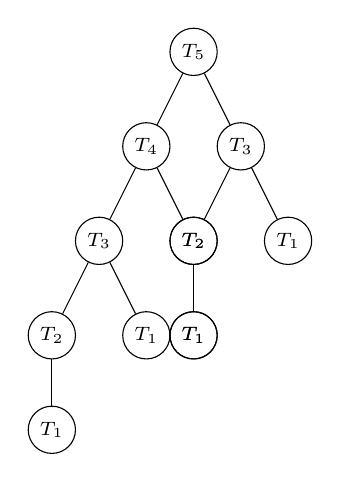
\begin{tikzpicture}[
    level distance=1.2cm,
    sibling distance=1.2cm,
    every node/.style={circle,draw,minimum size=6mm,inner sep=1pt,font=\scriptsize}
]
\node {$T_5$}
    child {node {$T_4$}
        child {node {$T_3$}
            child {node {$T_2$}
                child {node {$T_1$}}
            }
            child {node {$T_1$}}
        }
        child {node {$T_2$}
            child {node {$T_1$}}
        }
    }
    child {node {$T_3$}
        child {node {$T_2$}
            child {node {$T_1$}}
        }
        child {node {$T_1$}}
    };
\end{tikzpicture}
\end{center}

Each node in $T(k)$ is the root of a unique Fibonacci subtree $T(j)$ for some $1 \leq j \leq k$.

\section{Green Hackenbush Equivalence}

\begin{theorem}
The subtree removal game on a rooted tree is equivalent to \textbf{Green Hackenbush} on the same tree with the root as the grounded vertex.
\end{theorem}

\begin{proof}
Each non-root node $v$ in the tree corresponds to the edge $(v, \mathrm{parent}(v))$ in the Hackenbush graph. Removing node $v$ and its subtree is equivalent to removing the edge from $v$ to its parent, which disconnects all edges in $v$'s subtree from the ground. The game ends when no edges remain (only the grounded root), and the player to move loses---matching the normal-play convention of Hackenbush.
\end{proof}

\section{Nim Values via the Colon Principle}

\begin{definition}
For Green Hackenbush on a tree, the \textbf{Colon Principle} states: at any vertex, multiple branches can be replaced by a single stalk whose length equals the XOR (nim-sum) of the individual branch nim values.
\end{definition}

\begin{definition}
Define $\mathrm{nim}(k)$ as the Hackenbush nim value of $T(k)$ viewed as a branch (including the edge connecting its root to the parent node):
\begin{align}
    \mathrm{nim}(0) &= 0 \quad \text{(empty tree)} \\
    \mathrm{nim}(1) &= 1 \quad \text{(single edge)} \\
    \mathrm{nim}(k) &= 1 + \bigl(\mathrm{nim}(k{-}1) \oplus \mathrm{nim}(k{-}2)\bigr) \quad \text{for } k \geq 2
\end{align}
where $\oplus$ denotes bitwise XOR.
\end{definition}

The overall \textbf{Grundy value} of the game on $T(k)$ is:
\[
    G(k) = \mathrm{nim}(k{-}1) \oplus \mathrm{nim}(k{-}2).
\]

If $G(k) \neq 0$, the first player has a winning strategy. If $G(k) = 0$, the second player wins and $f(k) = 0$.

\begin{table}[h]
\centering
\begin{tabular}{r|rr|r}
\toprule
$k$ & $\mathrm{nim}(k)$ & $G(k)$ & $f(k)$ \\
\midrule
1 & 1 & 0 & 0 \\
2 & 2 & 1 & 1 \\
3 & 4 & 3 & 1 \\
4 & 7 & 6 & 1 \\
5 & 4 & 3 & 1 \\
6 & 4 & 3 & 3 \\
7 & 1 & 0 & 0 \\
8 & 6 & 5 & 7 \\
9 & 8 & 7 & 11 \\
10 & 15 & 14 & 17 \\
\bottomrule
\end{tabular}
\caption{Nim values, Grundy values, and winning move counts for small $k$.}
\end{table}

\section{Counting Winning First Moves}

A first move is \textbf{winning} if the resulting game state has Grundy value~0.

\begin{definition}
Let $h(k, t)$ denote the number of non-root nodes in $T(k)$ whose removal changes $\mathrm{nim}(k)$ to $t$.
\end{definition}

\begin{lemma}
The function $h$ satisfies the recurrence for $k \geq 2$:
\begin{align}
    h(k, t) &= [t = 1 + \mathrm{nim}(k{-}2)] \label{eq:caseA} \\
    &+ [k{-}2 \geq 1] \cdot [t = 1 + \mathrm{nim}(k{-}1)] \label{eq:caseB} \\
    &+ h\bigl(k{-}1,\; (t{-}1) \oplus \mathrm{nim}(k{-}2)\bigr) \quad \text{if } t \geq 1 \label{eq:caseC} \\
    &+ [k{-}2 \geq 1] \cdot h\bigl(k{-}2,\; (t{-}1) \oplus \mathrm{nim}(k{-}1)\bigr) \quad \text{if } t \geq 1 \label{eq:caseD}
\end{align}
with base cases $h(0, t) = h(1, t) = 0$ for all $t$.
\end{lemma}

The four terms correspond to:
\begin{enumerate}
    \item[\eqref{eq:caseA}] Removing the root of $T(k{-}1)$ (left child of root).
    \item[\eqref{eq:caseB}] Removing the root of $T(k{-}2)$ (right child of root).
    \item[\eqref{eq:caseC}] Removing a non-root node inside $T(k{-}1)$.
    \item[\eqref{eq:caseD}] Removing a non-root node inside $T(k{-}2)$.
\end{enumerate}

The answer is then:
\[
    f(k) = [\mathrm{nim}(k{-}2) = 0] + [\mathrm{nim}(k{-}1) = 0] + h(k{-}1,\, \mathrm{nim}(k{-}2)) + h(k{-}2,\, \mathrm{nim}(k{-}1)).
\]

\section{Implementation}

We store $h(k, \cdot)$ as a hash map from target nim values to counts. Only $h(k{-}1)$ and $h(k{-}2)$ are needed at each step (rolling storage). All counts are reduced modulo $10^{18}$.

\begin{algorithm}[h]
\caption{Compute $f(K) \bmod 10^{18}$}
\begin{algorithmic}[1]
\State Compute $\mathrm{nim}[0..K]$ using the recurrence
\State $h_{-2} \gets \{\},\; h_{-1} \gets \{\}$
\For{$k = 2$ \textbf{to} $K$}
    \State $h_k \gets \{\}$
    \State $h_k[1 + \mathrm{nim}[k{-}2]]\ {+}{=}\ 1$ \Comment{Case A}
    \If{$k{-}2 \geq 1$}
        \State $h_k[1 + \mathrm{nim}[k{-}1]]\ {+}{=}\ 1$ \Comment{Case B}
    \EndIf
    \ForAll{$(t', c) \in h_{-1}$} \Comment{Case C}
        \State $h_k[1 + (t' \oplus \mathrm{nim}[k{-}2])]\ {+}{=}\ c$
    \EndFor
    \If{$k{-}2 \geq 1$}
        \ForAll{$(t', c) \in h_{-2}$} \Comment{Case D}
            \State $h_k[1 + (t' \oplus \mathrm{nim}[k{-}1])]\ {+}{=}\ c$
        \EndFor
    \EndIf
    \State $h_{-2} \gets h_{-1},\; h_{-1} \gets h_k$
\EndFor
\State $f \gets [\mathrm{nim}[K{-}2]{=}0] + [\mathrm{nim}[K{-}1]{=}0] + h_{-1}[\mathrm{nim}[K{-}2]] + h_{-2}[\mathrm{nim}[K{-}1]]$
\State \Return $f \bmod 10^{18}$
\end{algorithmic}
\end{algorithm}

\section{Complexity}

\begin{itemize}
    \item \textbf{Time}: $O(K \cdot D)$ where $D \sim O(K)$ is the dictionary size per level, giving $O(K^2)$ overall.
    \item \textbf{Space}: $O(D) \sim O(K)$ for the two rolling dictionaries.
\end{itemize}

For $K = 10{,}000$, the dictionary sizes reach ${\sim}79{,}000$ entries at the final step, and the total computation involves ${\sim}5 \times 10^8$ operations.

\section{Answer}

\[
\boxed{438505383468410633}
\]

\end{document}
